\chapter{Landing Gear}

\section{Contact Point}

Landing gear contact point is considered to be an intersection of the ground plane and the line segment with the beginning at the strut attachment point and the end at the tire bottom.

\begin{figure}
  \centering
  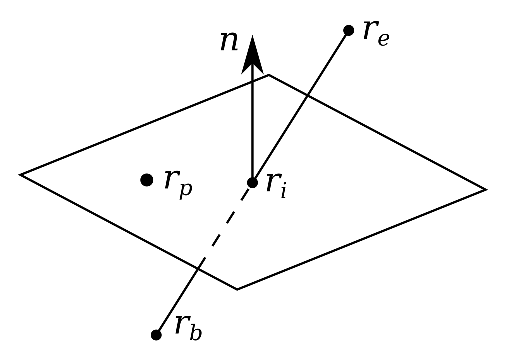
\includegraphics[width=80mm]{eps/segment_plane_intersection.eps}
  \caption{Segment-plane intersection}
\end{figure}

Intersection of a line segment and a plane can be calculated using following expression: \cite{ORourke1998}
\begin{equation}
  \label{eq-lg-intersection}
  u =
  \frac
  { \vec n \cdot \left( {\vec r}_p - {\vec r}_b \right) }
  { \vec n \cdot \left( {\vec r}_e - {\vec r}_b \right) }
\end{equation}

Where:
\begin{description}[align=right,labelwidth=1cm]
  \item [$\vec n$]     --- unit vector normal to the plane
  \item [${\vec r}_b$] --- position vector of the line segment beginning
  \item [${\vec r}_e$] --- position vector of the line segment end
  \item [${\vec p}_b$] --- position vector of any point on the plane
  \item [$u$]          --- normalized coordinate of intersection point along line segment
\end{description}

If $0 \leq u \leq 1$ then intersection point is within line segment and its coordinates are given by the following formula:
\begin{equation}
  \vec r = {\vec r}_b = u \left( {\vec r}_e - {\vec r}_r \right)
\end{equation}

If denominator of expression (\ref{eq-lg-intersection}) is zero then the line segment is parallel to the plane. If both numerator and denominator are zero then the line segment lies on the plane.

\section{Forces and Moments}

Forces generated by the landing gear can be divided into:
\begin{itemize}
  \item[---] normal to the ground plane forces due to struts and tires deflection,
  \item[---] tangent to the ground plane forces due to friction between tires and the ground.
\end{itemize}

Normal forces are the sum of forces due to spring and damper while tangent force are caused by static or kinetic friction and optional rolling friction and are given as follows: \cite{ResnickHalliday2011}
\begin{align}
  F_N &= kx + c \dot x \\
  F_T &= \mu F_N
\end{align}

\begin{table}[h!]
  \begin{center}
    \begin{tabular}{ l | c | c }
      \toprule
      \textbf{Surface} & \textbf{Static friction coefficient} & \textbf{Kinetic friction coefficient} \\ \midrule
      Concrete (dry) &  0.8 - 1.0  &  0.7 - 0.8  \\
      Concrete (wet) &  0.6 - 0.8  &  0.5 - 0.6  \\
      Tarmac (dry)   &  0.7 - 0.8  &  0.6 - 0.7  \\
      Tarmac (wet)   &  0.4 - 0.5  &  0.3 - 0.4  \\
      Dirt (dry)     &  0.5 - 0.6  &  0.2 - 0.3  \\
      Dirt (wet)     &  0.3 - 0.4  &  0.2 - 0.3  \\
      Snow           &  0.1 - 0.4  &  0.2 - 0.3  \\
      Ice            & 0.05 - 0.15 & 0.05 - 0.10 \\
      \bottomrule
    \end{tabular}
    \caption{Static and kinetic friction coefficients \cite{Studzinski1980} }
  \end{center}
\end{table}

\begin{table}[h!]
  \begin{center}
    \begin{tabular}{ l | c }
      \toprule
      \textbf{Surface} & \textbf{Rolling friction coefficient} \\ \midrule
      Tarmac   &  0.010 - 0.012 \\
      Concrete &  0.012 - 0.015 \\
      Dirt     &  0.030 - 0.140 \\
      \bottomrule
    \end{tabular}
    \caption{Static and kinetic friction coefficients \cite{Studzinski1980} }
  \end{center}
\end{table}
